% 本模板根据中国科学院大学本科生公共必修课程《基础物理实验》Word模板格式编写
% 本模板由Shing-Ho Lin和Jun-Xiong Ji于2022年9月共同完成, 旨在方便LaTeX原教旨主义者和被Word迫害者写实验报告, 避免Word文档因插入过多图与公式造成卡顿. 
% 如有任何问题, 请联系: linchenghao21@mails.ucas.ac.cn
% This is the LaTeX template for experiment report of Experimental Physics courses, based on its provided Word template. 
% This template is completed by the joint collabration of Shing-Ho Lin and Junxiong Ji in September 2022. 
% Adding numerous pictures and equations leads to unsatisfying experience in Word. Therefore LaTeX is better. 
% Feel free to contact us via: linchenghao21@mails.ucas.ac.cn

\documentclass[UTF8]{article}
\usepackage[UTF8]{ctex} % 支持中文的LaTeX宏包
\usepackage[a4paper]{geometry}
\geometry{left=2.0cm,right=2.0cm,top=2.5cm,bottom=2.5cm}
\usepackage{amsmath,amsfonts,graphicx,subfigure,amssymb,bm,amsthm,mathrsfs,mathtools,breqn} % 数学公式和符号的宏包集合
\usepackage{algorithm,algorithmicx} % 算法和伪代码的宏包
\usepackage[noend]{algpseudocode} % 算法和伪代码的宏包
\usepackage{fancyhdr} % 自定义页眉页脚的宏包
\usepackage[framemethod=TikZ]{mdframed} % 创建带边框的框架的宏包
\usepackage{fontspec} % 字体设置的宏包
\usepackage{adjustbox} % 调整盒子大小的宏包
\usepackage{fontsize} % 设置字体大小的宏包
\usepackage{tikz,xcolor} % 绘制图形和使用颜色的宏包
\usepackage{multicol} % 多栏排版的宏包
\usepackage{multirow} % 表格中合并单元格的宏包
\usepackage{pdfpages} % 插入PDF文件的宏包
\RequirePackage{listings} % 在文档中插入源代码的宏包
\RequirePackage{xcolor} % 定义和使用颜色的宏包
\usepackage{wrapfig} % 文字绕排图片的宏包
\usepackage{bigstrut,multirow,rotating} % 支持在表格中使用特殊命令的宏包
\usepackage{booktabs} % 创建美观的表格的宏包
\usepackage{circuitikz} % 绘制电路图的宏包

\definecolor{dkgreen}{rgb}{0,0.6,0}
\definecolor{gray}{rgb}{0.5,0.5,0.5}
\definecolor{mauve}{rgb}{0.58,0,0.82}
\lstset{
  frame=tb,
  aboveskip=3mm,
  belowskip=3mm,
  showstringspaces=false,
  columns=flexible,
  framerule=1pt,
  rulecolor=\color{gray!35},
  backgroundcolor=\color{gray!5},
  basicstyle={\small\ttfamily},
  numbers=none,
  numberstyle=\tiny\color{gray},
  keywordstyle=\color{blue},
  commentstyle=\color{dkgreen},
  stringstyle=\color{mauve},
  breaklines=true,
  breakatwhitespace=true,
  tabsize=3,
}

% 轻松引用, 可以用\cref{}指令直接引用, 自动加前缀. 
% 例: 图片label为fig:1
% \cref{fig:1} => Figure.1
% \ref{fig:1}  => 1
\usepackage[capitalize]{cleveref}
% \crefname{section}{Sec.}{Secs.}
\Crefname{section}{Section}{Sections}
\Crefname{table}{Table}{Tables}
\crefname{table}{Table.}{Tabs.}

\setmainfont{Palatino Linotype}
\setCJKmainfont{SimHei}
 \setCJKsansfont{Songti}
 \setCJKmonofont{SimSun}
\punctstyle{kaiming}
% 偏好的几个字体, 可以根据需要自行加入字体ttf文件并调用

\renewcommand{\emph}[1]{\begin{kaishu}#1\end{kaishu}}

%改这里可以修改实验报告表头的信息
\newcommand{\experiName}{虚拟仪器}
\newcommand{\supervisor}{石澔玙}
\newcommand{\name}{张欣培}
\newcommand{\studentNum}{2022K8009922001}
\newcommand{\class}{01}
\newcommand{\group}{10}
\newcommand{\seat}{3}
\newcommand{\dateYear}{2023}
\newcommand{\dateMonth}{11}
\newcommand{\dateDay}{6}
\newcommand{\room}{教702}
\newcommand{\others}{$\square$}
%% 如果是调课、补课, 改为: $\square$\hspace{-1em}$\surd$
%% 否则, 请用: $\square$
%%%%%%%%%%%%%%%%%%%%%%%%%%%

\begin{document}
%若需在页眉部分加入内容, 可以在这里输入
% \pagestyle{fancy}
% \lhead{\kaishu 测试}
% \chead{}
% \rhead{}

\begin{center}
    \LARGE \bf 《\, 基\, 础\, 物\, 理\, 实\, 验\, 》\, 实\, 验\, 报\, 告
\end{center}

\begin{center}
    \noindent \emph{实验名称}\underline{\makebox[25em][c]{\experiName}}
    \emph{指导教师}\underline{\makebox[8em][c]{\supervisor}}\\
    \emph{姓名}\underline{\makebox[6em][c]{\name}} 
    % 如果名字比较长, 可以修改box的长度"6em"
    \emph{学号}\underline{\makebox[10em][c]{\studentNum}}
    \emph{分班分组及座号} \underline{\makebox[5em][c]{\class \ -\ \group \ -\ \seat }\emph{号}} (\emph{例}:\, 1\,-\,04\,-\,5\emph{号})\\
    \emph{实验日期} \underline{\makebox[3em][c]{\dateYear}}\emph{年}
    \underline{\makebox[2em][c]{\dateMonth}}\emph{月}
    \underline{\makebox[2em][c]{\dateDay}}\emph{日}
    \emph{实验地点}\underline{{\makebox[4em][c]\room}}
    \emph{调课/补课} \underline{\makebox[3em][c]{\others\ 是}}
    \emph{成绩评定} \underline{\hspace{5em}}
    {\noindent}
    \rule[8pt]{17cm}{0.2em}
\end{center}

\begin{center}
    \Large \bf 第一部分\qquad 实验内容
\end{center}

\section{实验目的}

\begin{enumerate}
    \item 了解虚拟仪器的概念;
    \item 了解图形化编程语言 LabVIEW ,学习简单的 LabVIEW 编程;
    \item 完成伏安法测电阻的虚拟仪器设计。
\end{enumerate}

\section{实验器材}

计算机(含操作系统,LabVIEW 2014软件),NI ELVIS $\uppercase\expandafter{\romannumeral2} ^+$教学实验室虚拟仪器套件,导线若干,元件盒一个(包括
 $100\Omega$ 标准电阻一个,待测电阻两个,二极管一个),热电偶等元件。

\section{实验原理}
\begin{enumerate}
    \item 虚拟仪器的硬件
    \newline \hspace*{2em}本实验使用的硬件平台是计算机,和美国国家仪器公司(National Instruments)的教学实验室虚拟仪器套件(Educational Laboratory Virtual Instrumentation Suite)$\uppercase\expandafter{\romannumeral2}^+ $(缩写为NI ELVIS$\uppercase\expandafter{\romannumeral2}^+ $)和自带的原型板(如图1)。
    虚拟仪器是一种基于计算机的自动化测试仪器系统。它利用通用计算机的强大计算处理功能,通过传感器和接口卡实现信号输入,用键盘、鼠标、显示器等计算机外设实现控制和显示功能。
    \begin{figure}[h]
        \centering
        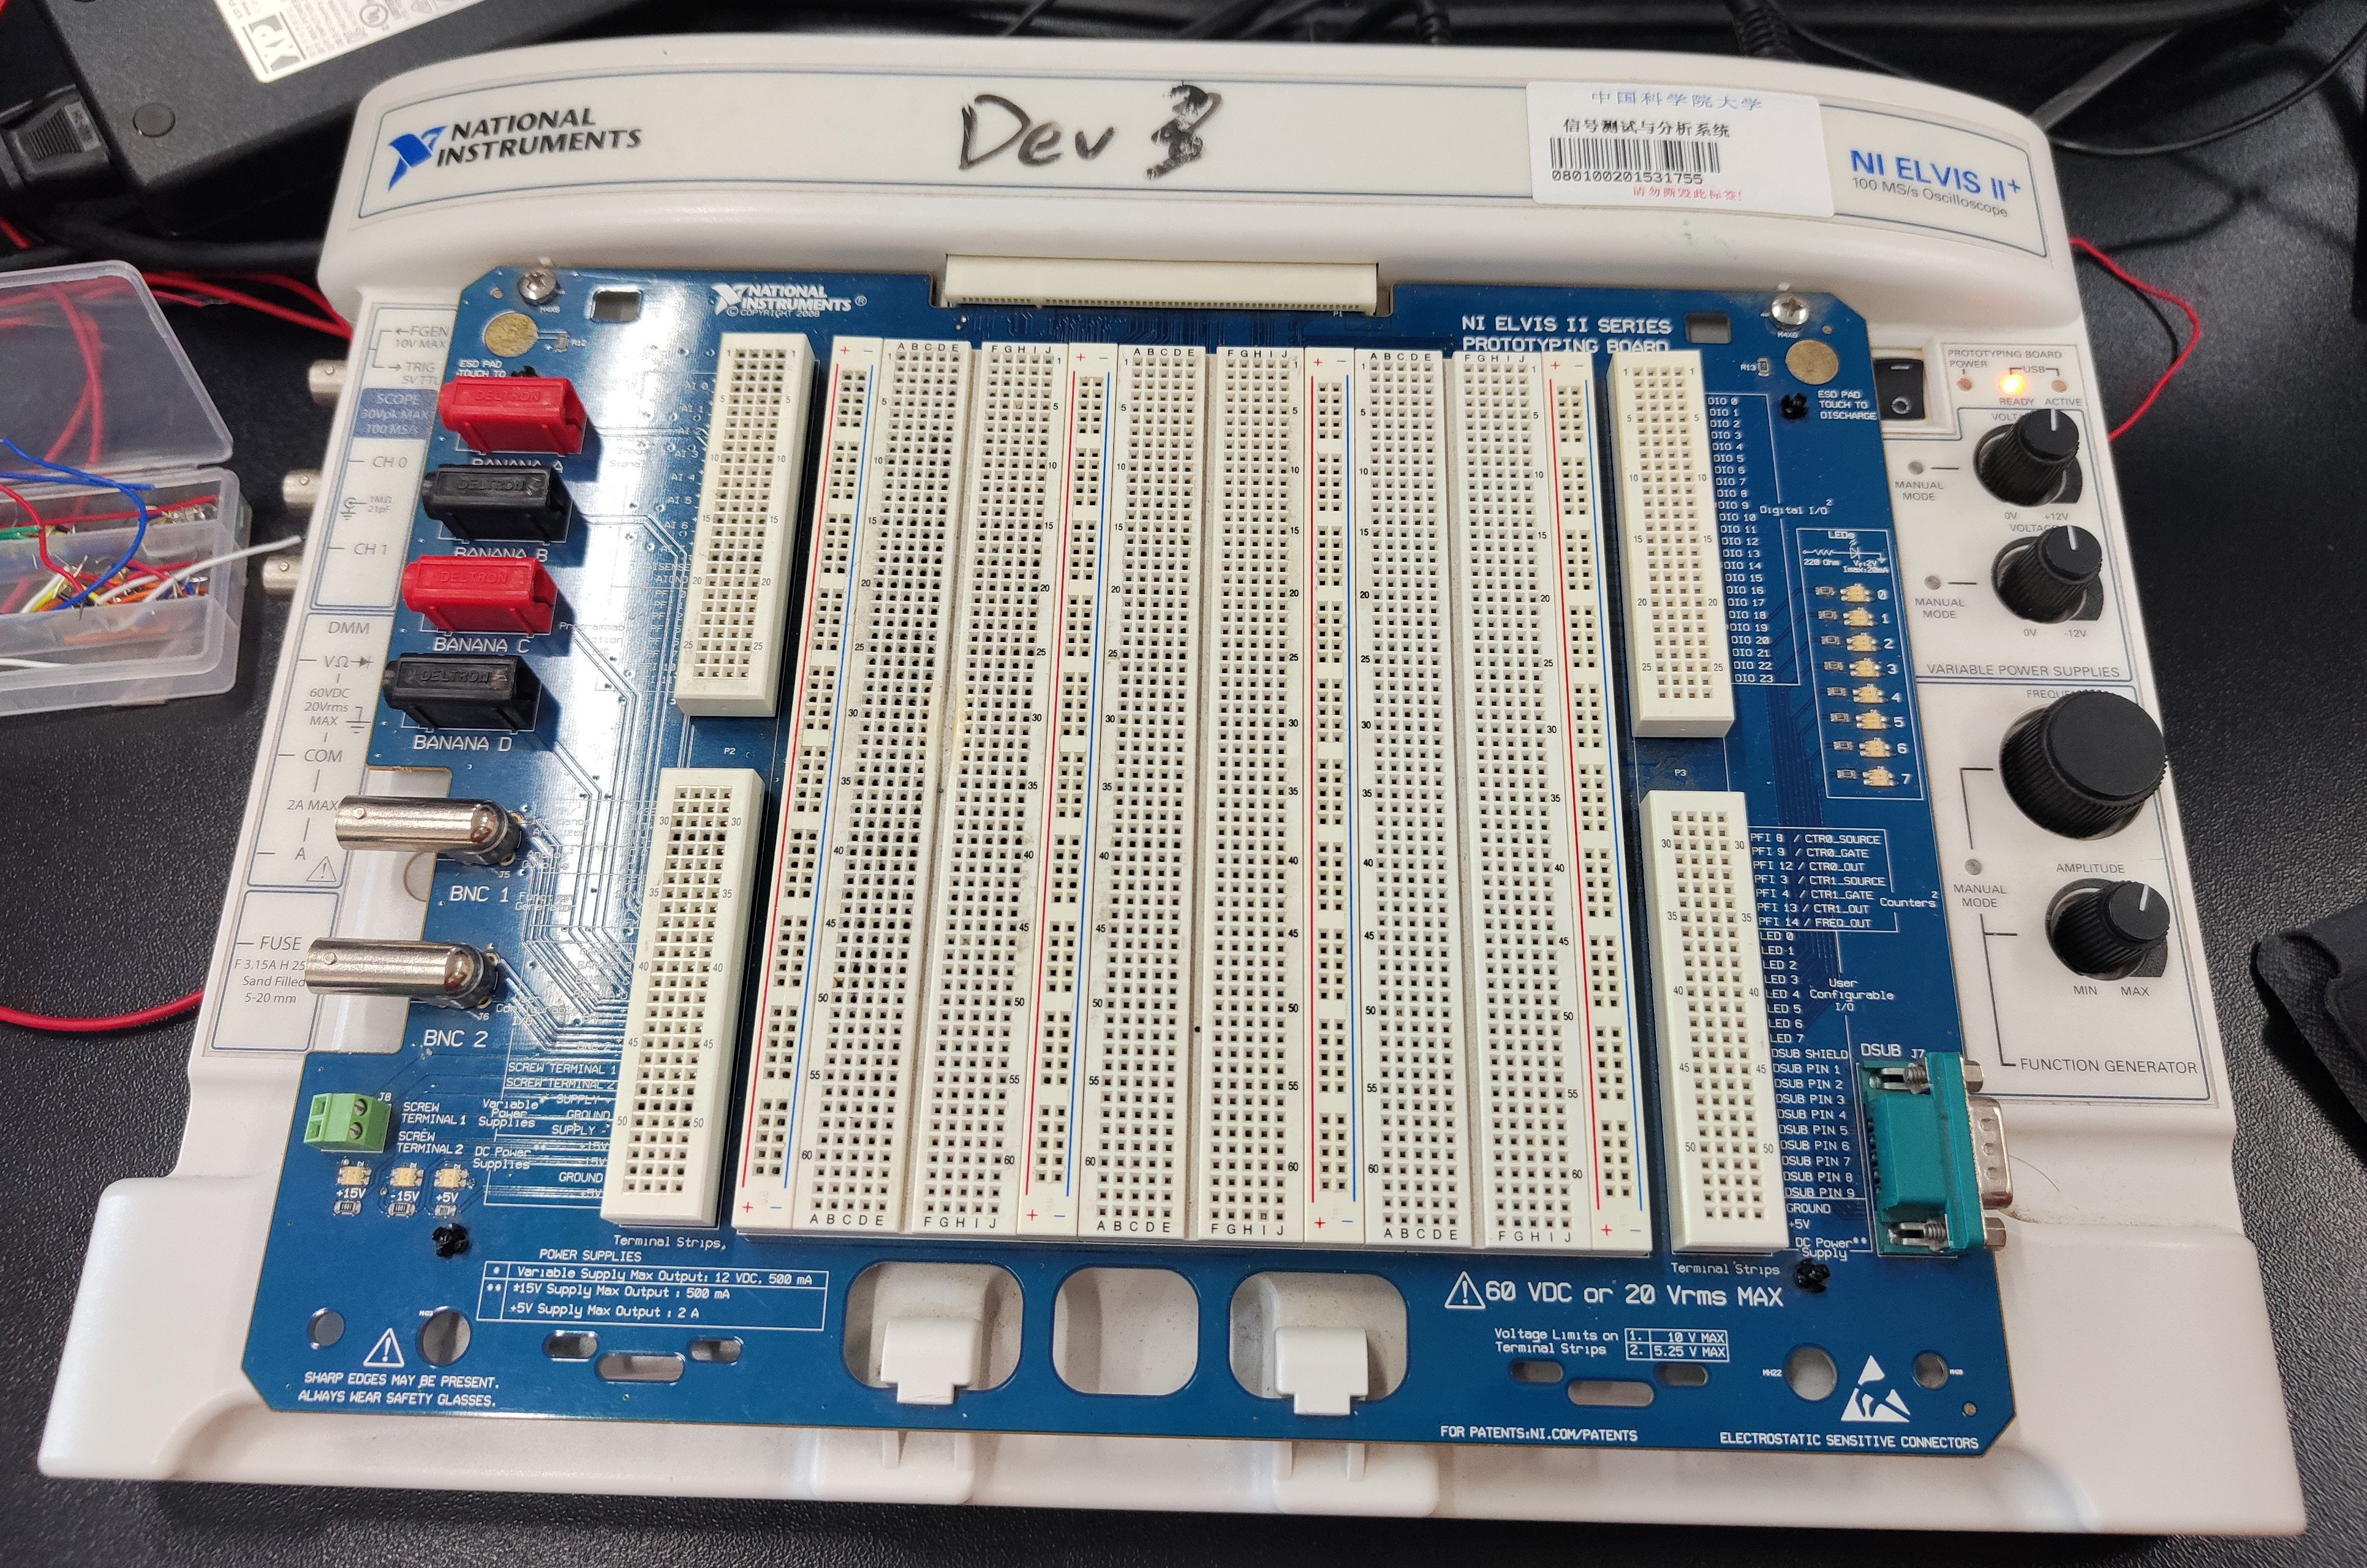
\includegraphics[width=13cm]{Fig/1.jpg}
        \caption{NI ELVIS$\uppercase\expandafter{\romannumeral2}^+$}
    \end{figure}
    \newline \hspace*{2em}虚拟仪器综合实验平台是开源的,可以在 LabVIEW 中进行定制,同时可以使用 LabVIEW Express $\uppercase\expandafter{\romannumeral6} $ 和 LabVIEW Signal Express 的步骤对设备进行编程。其可连接其他设备。
    \item 虚拟仪器的软件
    \newline \hspace*{2em}本实验使用的用于虚拟仪器系统设计的软件开发平台是LabVIEW (laboratory virtual instrument engineering workbench)。它将计算机数据分析和显示能力与仪器驱动程序整合在一起,为针对仪器的编程提供了很大的便利。它是一种图形化编程语言,易于上手。
    \item 利用虚拟仪器测量伏安特性
    \newline \hspace*{2em}测量伏安特性曲线实验我们从高中物理就不陌生。本实验通过编程利用元器件,由导线相连。本实验中利用一个模拟输出通道为整个测量电路供电,利用两个模拟输入通道分别测量总电压和标准电阻上的电压;利用测量得到的电压数值和标准电阻数值就可以得到电路中的电流以及待测电阻上的电压。
    \begin{figure}[H]
        \centering
        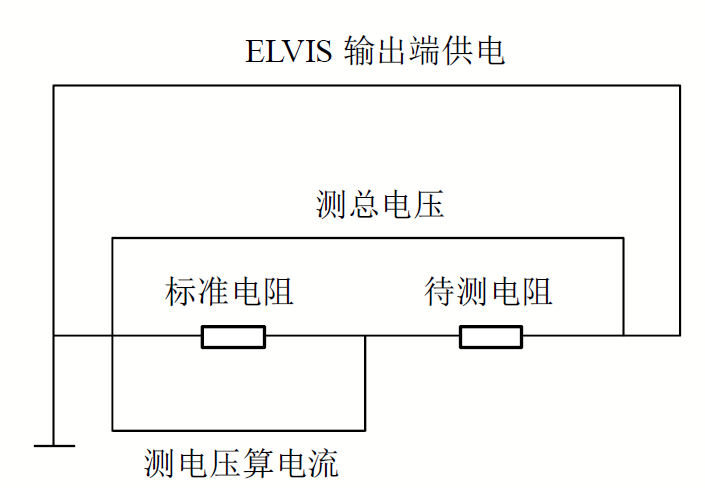
\includegraphics[width=8cm]{Fig/2.png}
        \caption{测伏安曲线电路}
    \end{figure}
    
\end{enumerate}


\section{实验内容}
\subsection{初步熟悉LabVIEW开发环境的基本操作和编程方法}
    此部分略过,具体操作将在后面实验中实现。鉴于不同软件操作不同,且本软件操作较为简单,无需叙述。
\subsection{创建一个温度测量程序}

\begin{enumerate}
    \item 如图3搭建模拟温度测量程序。
    \item 选择前面板窗口,运行 VI 程序。点击连续运行按钮,使程序运行于连续运行模式。改变采
    集的电压控件输入值(比如在 0.5-2 之间的任意值)和温度值单位,观察程序运行情况,并解
    释程序每部分的功能。再点击连续运行按钮,停止程序运行。(注:本实验中没有连接真实的测温计,由虚拟输入“采集的电压”模拟输入,因此也无具体的实验结果,只有模拟输入的数据转换。)
    \item 用文件菜单的保存功能(或 <Ctrl+S>快捷键)保存上述文件。关闭程序。
\end{enumerate}
\begin{figure}[H]
    \centering
    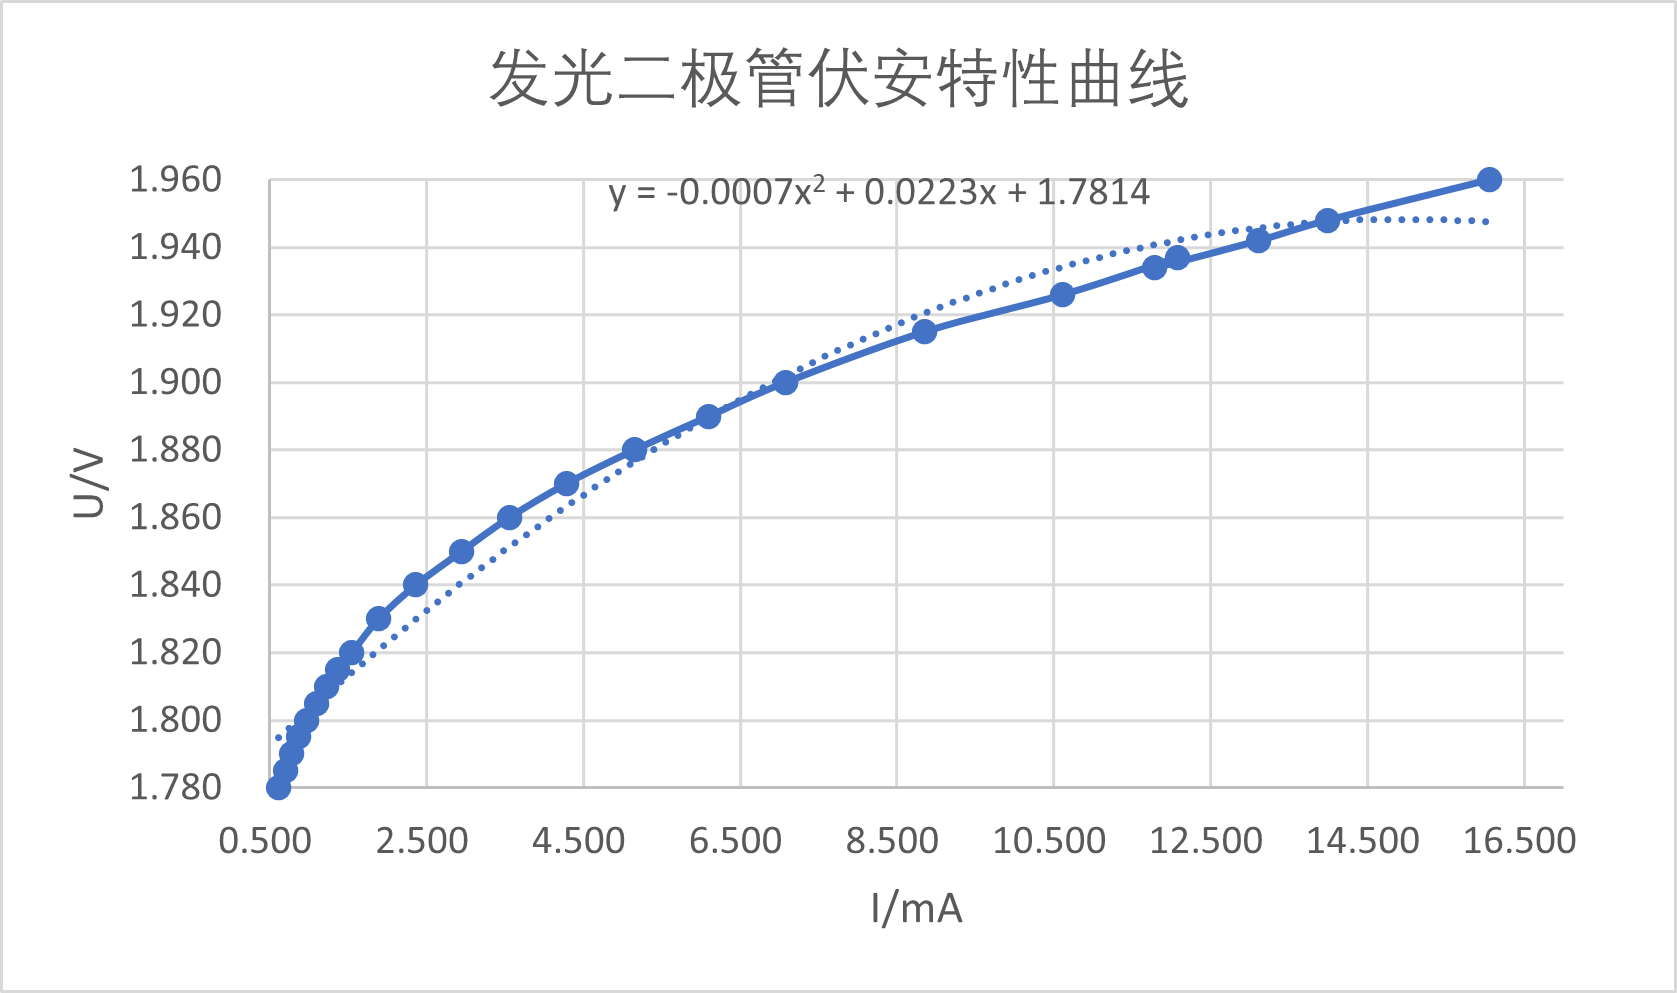
\includegraphics[width=17cm]{Fig/3.png}
    \caption{温度测量程序}
\end{figure}
\subsection{创建一个电压输出和采集的程序}
\begin{figure}[H]
    \centering
    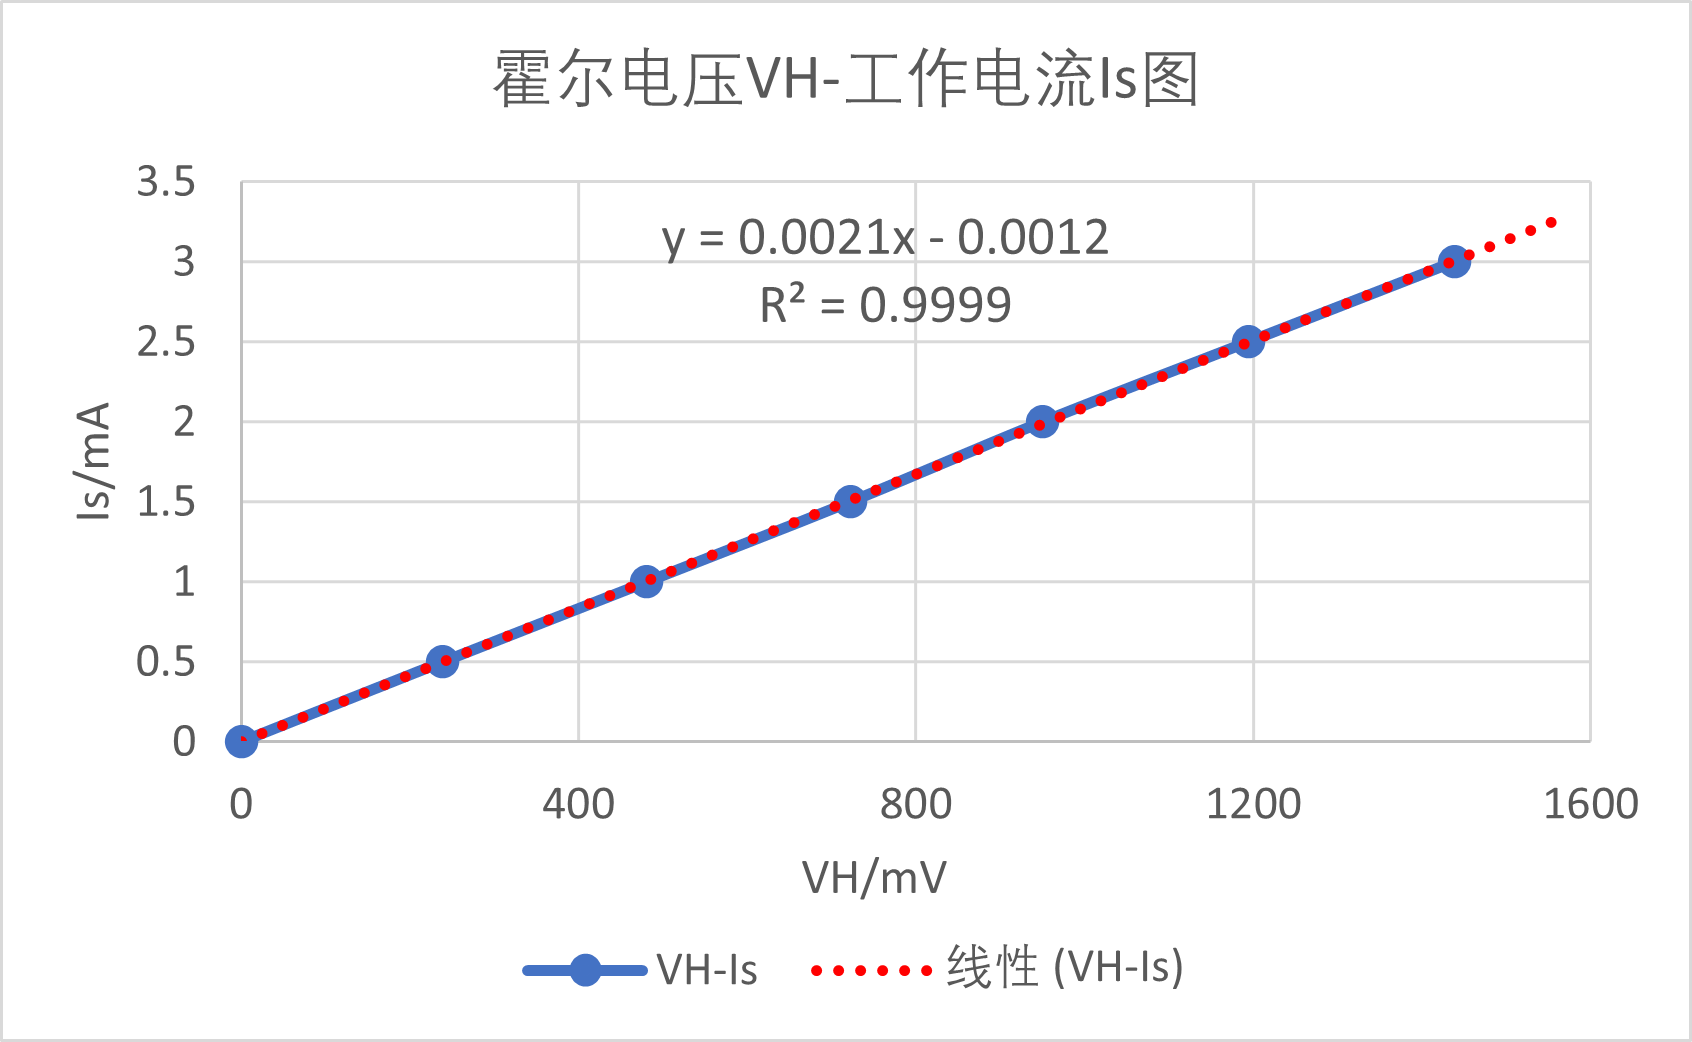
\includegraphics[width=17cm]{Fig/4.png}
    \caption{电压输出和采集的程序}
\end{figure}
\begin{enumerate}
    \item 实验过程
    \begin{enumerate}
        \item 如图4搭建模拟温度测量程序。
        \item 打开ELVIS 电源和原型板电源。在前面板上设置输出通道为 Dev3/ao0 ,输入通道为 Dev3/ai0 。
        在原型板上用导线连接模拟输出( Analog Outputs ))“AO 0”端和模拟输入( Analog Input Signals)
        “AI 0 +”端,将 “AI 0 -”端和接地端 “AIGND” 用导线连接。
        在前面板窗口,运行 VI 程序。改变输出电压,观察测量电压的变化。可点击停止按钮,观察程序运行情况。
        \item 保存上述文件。关闭程序。
    \end{enumerate}
    \item 实验结果
    \begin{enumerate}
        \item 如图4,输出电压3V,输入电压2.999V,在测量误差允许范围内。
    \end{enumerate}
\end{enumerate}
\subsection{用虚拟仪器测量伏安特性}
\begin{figure}[H]
    \centering
    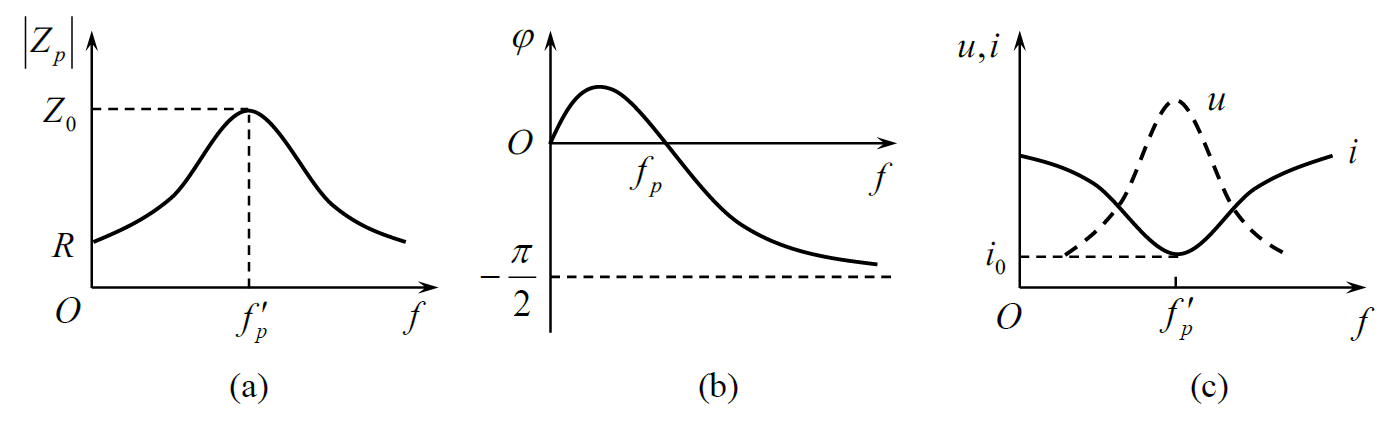
\includegraphics[width=17cm]{Fig/5.png}
    \caption{测量伏安特性的程序框图}
\end{figure}
\begin{enumerate}
    \item 实验步骤
    \begin{enumerate}
        \item 如图5,6搭建模拟伏安特性曲线测量程序。(注:相较于实验说明所给的电路图,增加了“瞬时总电压”和“瞬时标准电阻电压”两模块,用来在测量时观测瞬时测量情况。同时,循环变量设为i+1,本程序i从0开始,这样能忽略掉输入电压为0V的测量。)
        \item 在ELVIS自带的原型板上正确连接电路。
        \item 再次检查前面板窗口中各参量设置情况,根据所测样本选择合适的测量数据点数和输出电压步长。(电路板最大电流$10mA$)标准电阻$100\Omega$,时间间隔$0.02s$。打开开关,运行程序。分别测量两个待测电阻的电阻值和稳压二极管的电阻值。
        \item 选择程序框图内的“数据”,右键导出数据为excel,处理数据。
        \item 保存上述文件。关闭程序。
    \end{enumerate}
    \begin{figure}[H]
        \begin{minipage}[t]{0.69\linewidth}
            \centering
            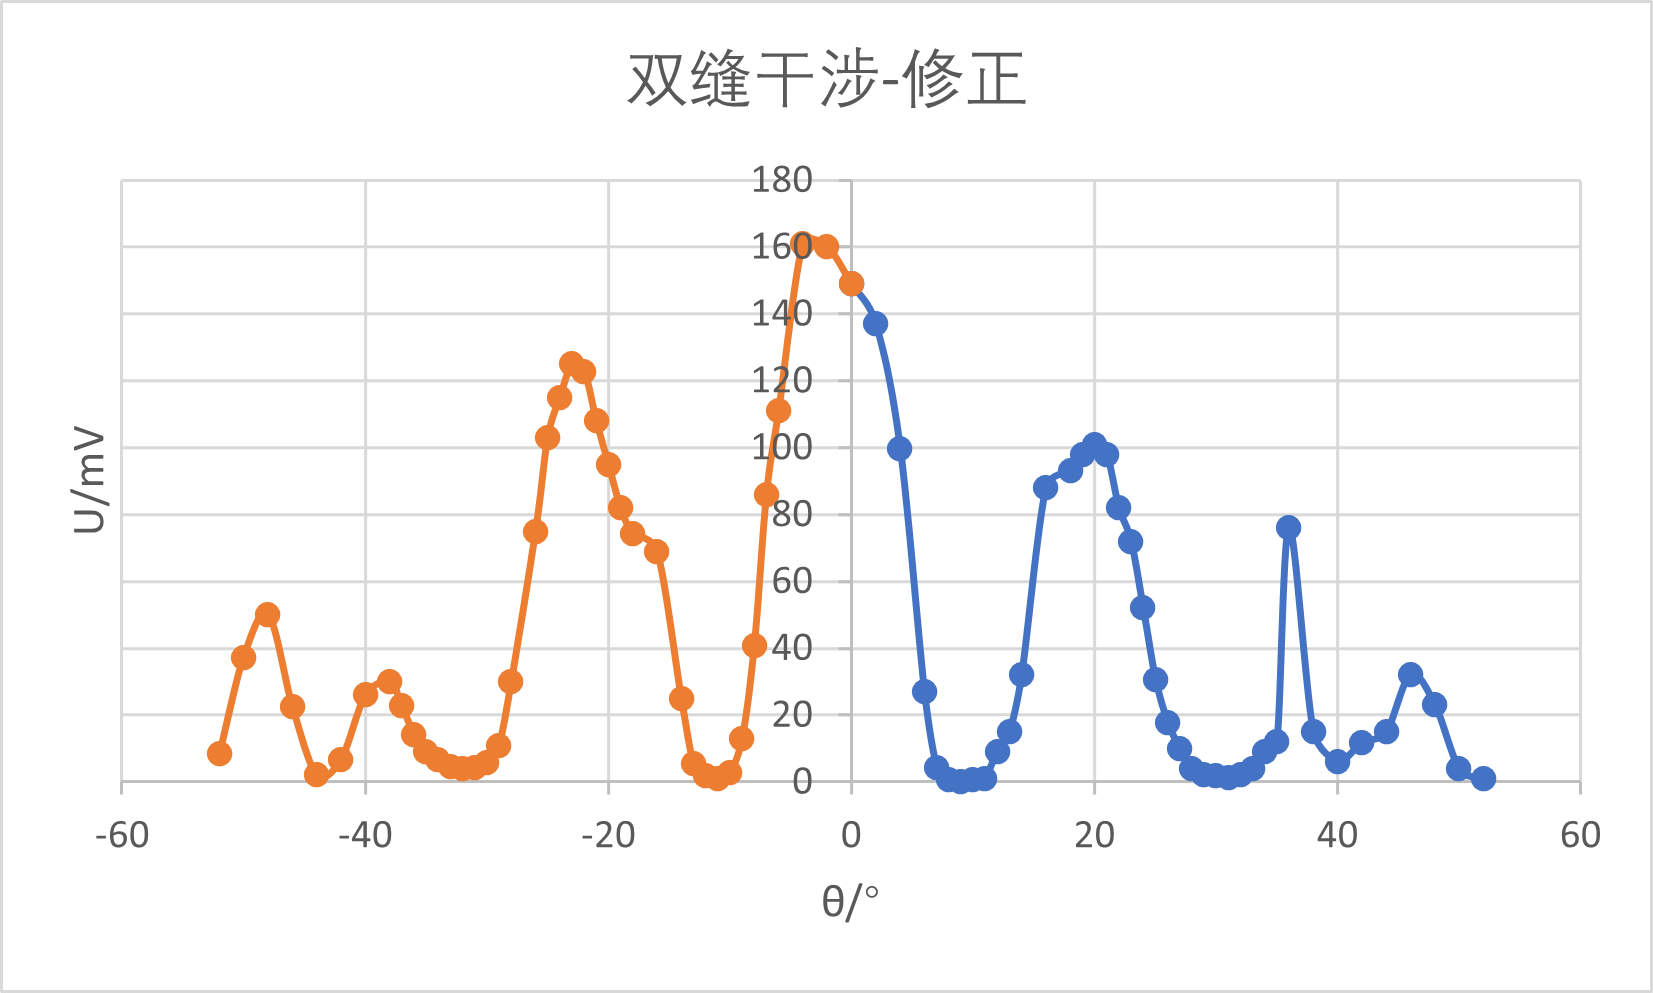
\includegraphics[width=11.5cm]{Fig/6.png}
            \caption{测量伏安特性的前面板($100\Omega$电阻)}
        \end{minipage}
        \begin{minipage}[t]{0.3\linewidth}
            \centering
            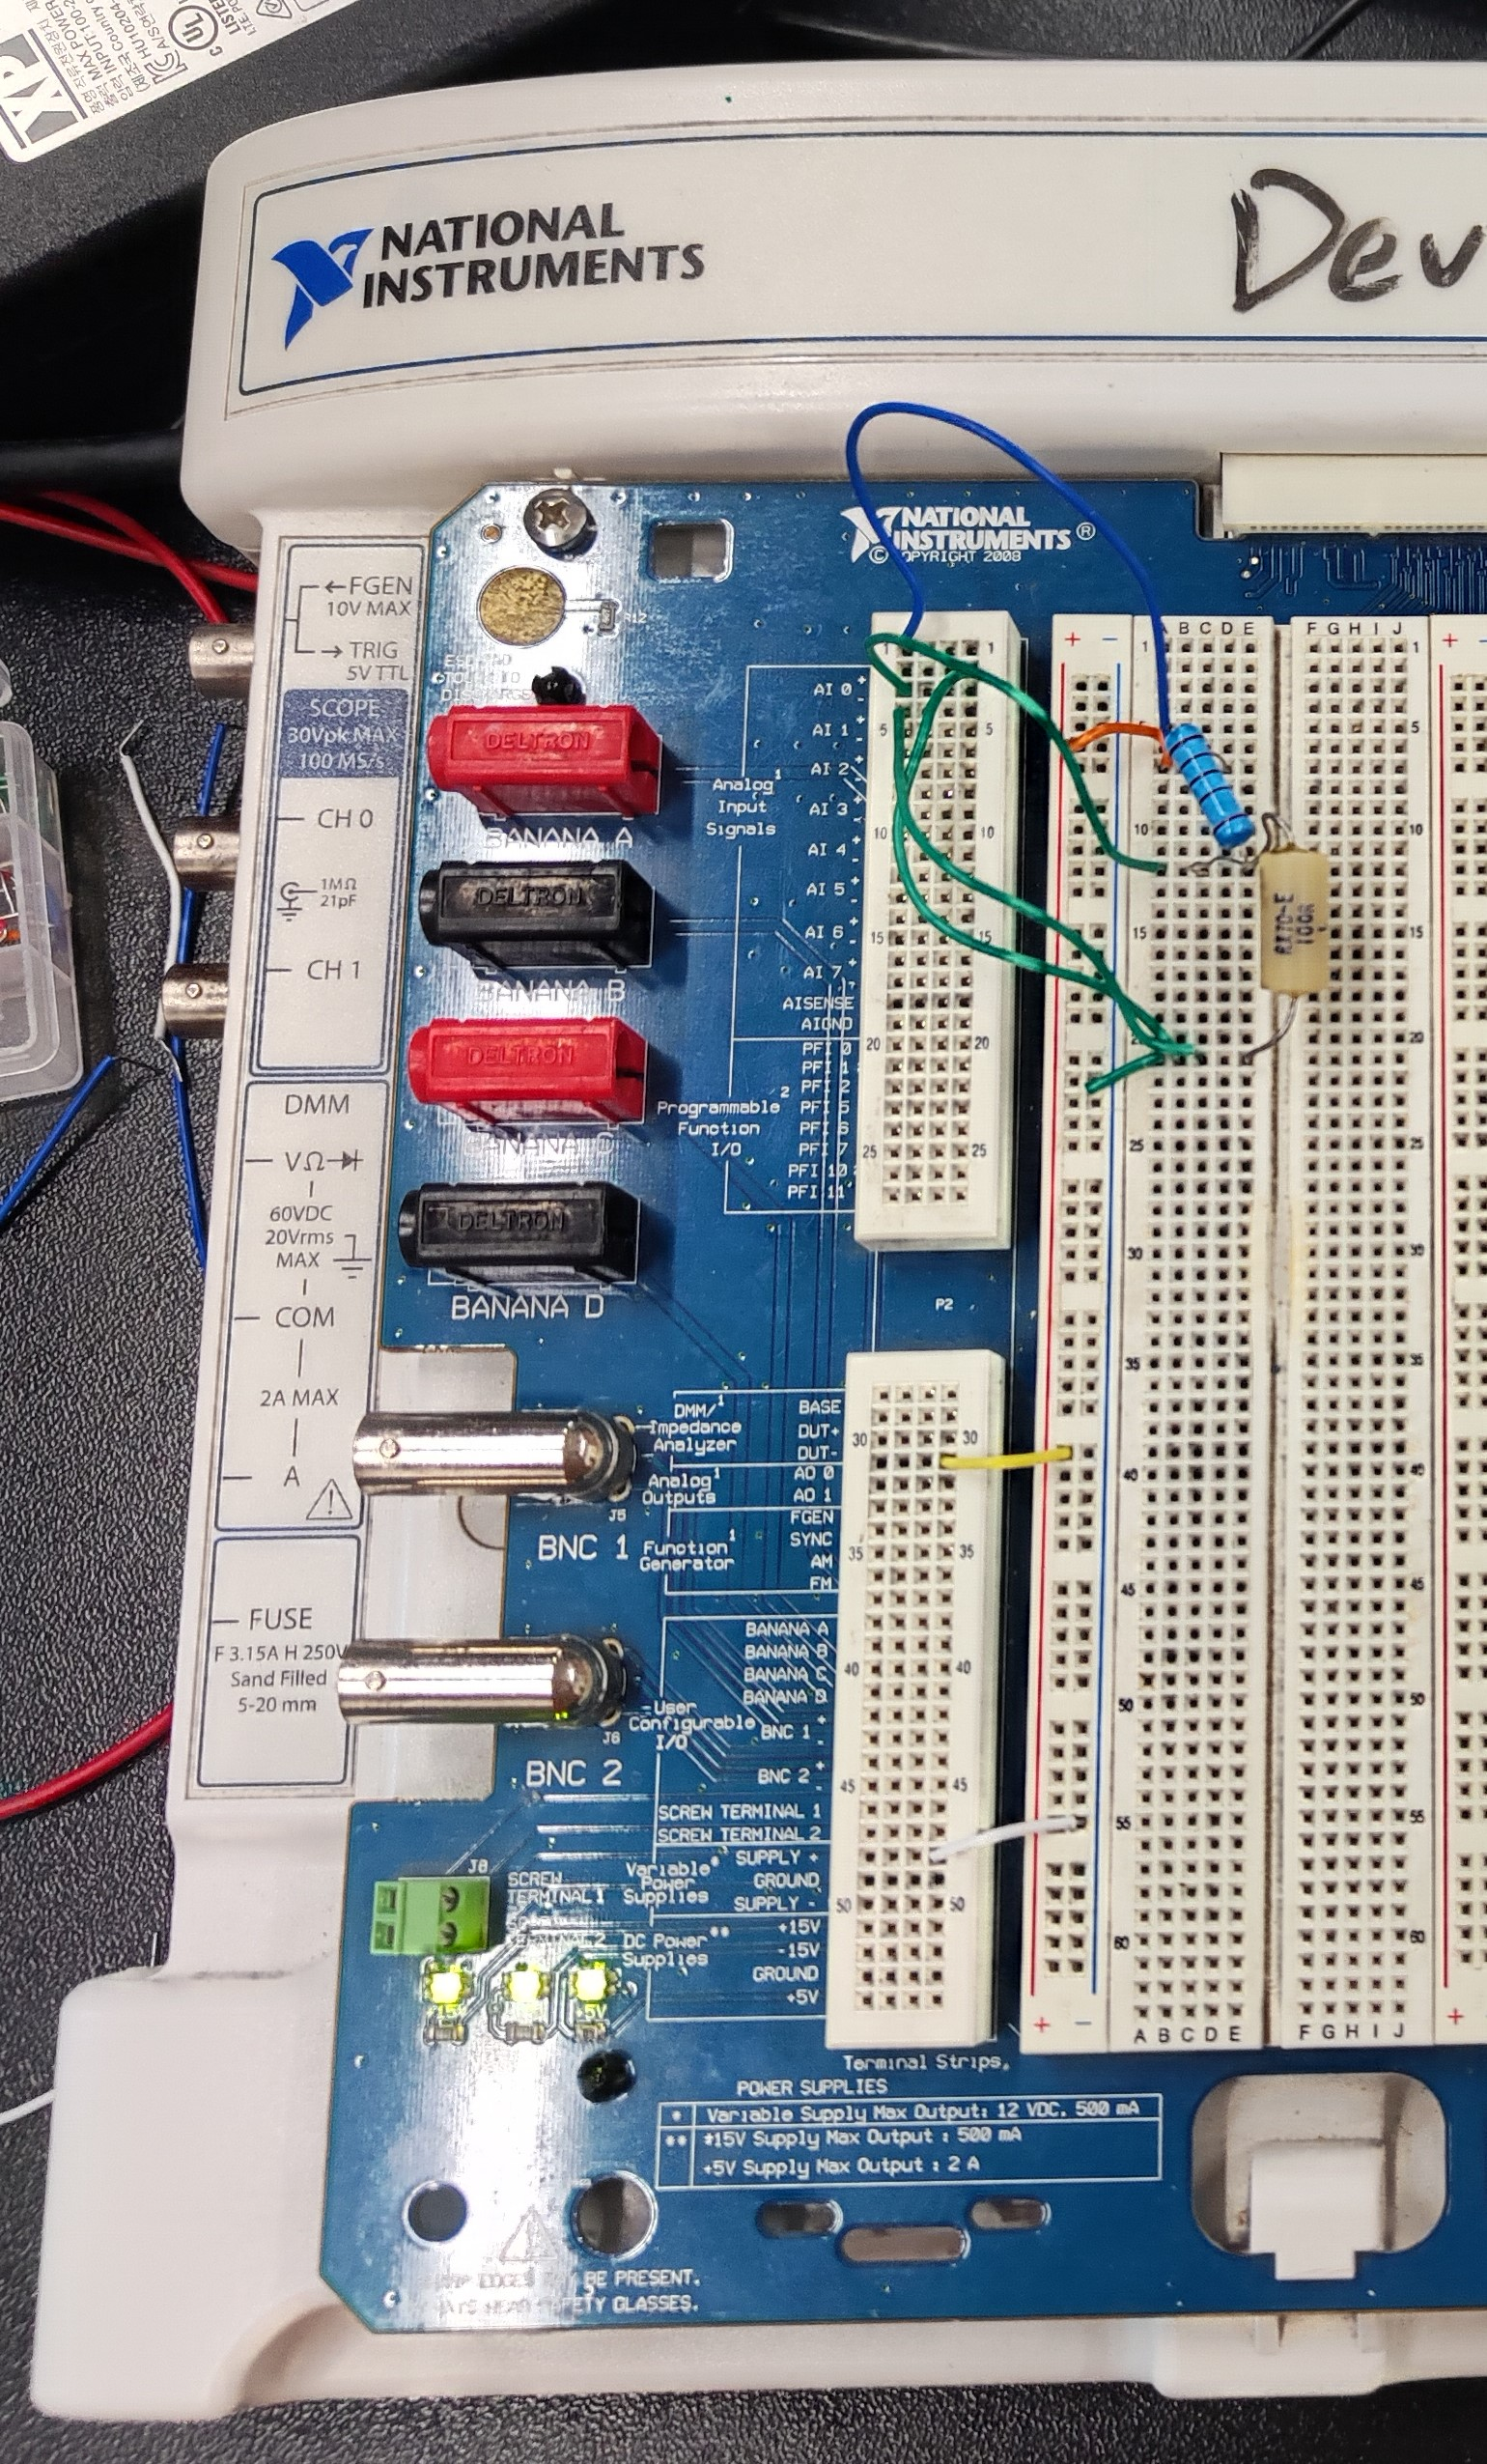
\includegraphics[width=5cm]{Fig/7.jpg}
            \caption{测量伏安特性的电路图(100$\Omega$电阻)}
        \end{minipage}
       
    \end{figure}
    \item 数据处理
    \begin{enumerate}
        \item $100\Omega$电阻伏安特性曲线
                % Table generated by Excel2LaTeX from sheet '99o-2'
        \begin{table}[H]
          \centering
          \caption{$100\Omega$电阻伏安特性数据}
            \begin{tabular}{|l|r|r|r|r|r|}\hline
            $U/V$    & 0.0151342 & 0.0218963 & 0.0334884 & 0.0434705 & 0.0537746 \\\hline
            $I/A$    & 0.000161048 & 0.000247989 & 0.00034459 & 0.000431531 & 0.000537793 \\\hline
            $U/V$    & 0.0602147 & 0.0708409 & 0.079535 & 0.0904831 & 0.101753 \\\hline
            $I/A$    & 0.000605414 & 0.000714895 & 0.000830816 & 0.000914537 & 0.000998258 \\\hline
            $U/V$    & 0.113023 & 0.121073 & 0.131056 & 0.141038 & 0.152952 \\\hline
            $I/A$    & 0.00114316 & 0.00120756 & 0.00132348 & 0.0014394 & 0.00155855 \\\hline
            $U/V$    & 0.161324 & 0.167764 & 0.177102 & 0.184508 & 0.195456 \\\hline
            $I/A$    & 0.00162939 & 0.00168735 & 0.00180005 & 0.00187733 & 0.00196105 \\\hline
            \end{tabular}%
          \label{tab:100Omega}%
        \end{table}%
        设置输出电压步长$0.08V$。如图8(a),Excel拟合直线所得值$R=99.262\Omega$,程序拟合值$R=99.26\Omega$。
        \item $10k\Omega$电阻伏安特性曲线
                % Table generated by Excel2LaTeX from sheet 'lvtemporary_653276'
        \begin{table}[H]
          \centering
          \caption{$10k\Omega$电阻伏安特性数据}
            \begin{tabular}{|l|r|r|r|r|r|}\hline
            U/V    & 0.47882 & 0.947658 & 1.41424 & 1.87632 & 2.33936 \\\hline
            I/A    & 5.16E-05 & 0.000106308 & 0.000144948 & 0.000196469 & 0.000241549 \\\hline
            U/V    & 2.80241 & 3.26191 & 3.72399 & 4.18575 & 4.64815 \\\hline
            I/A    & 0.00028019 & 0.00033815 & 0.000383231 & 0.000428311 & 0.000463732 \\\hline
            U/V    & 5.10604 & 5.5678 & 6.02828 & 6.49101 & 6.95438 \\\hline
            I/A    & 0.000524913 & 0.000566773 & 0.000615074 & 0.000660154 & 0.000705235 \\\hline
            U/V    & 7.41583 & 7.87631 & 8.33872 & 8.79727 & 9.25099 \\\hline
            I/A    & 0.000743875 & 0.000801836 & 0.000843696 & 0.000891997 & 0.000933858 \\\hline
            \end{tabular}%
          \label{tab:10kOmega}%
        \end{table}%
        设置输出电压步长$0.5V$。如图8(b),Excel拟合直线所得值$R=9945.7\Omega$,程序拟合值$R=9945.74\Omega$。

        \item 发光二极管伏安特性曲线
                % Table generated by Excel2LaTeX from sheet 'lvtemporary_725271'
        \begin{table}[H]
          \centering
          \caption{发光二极管伏安特性数据}
            \begin{tabular}{|l|r|r|r|r|r|r|}\hline
            $U/V$ & 0.29077 & 0.592487 & 0.893239 & 1.19303 & 1.49088 & 1.73206 \\\hline
            $I/A$ & 1.29E-05 & 3.27E-06 & 3.27E-06 & 3.27E-06 & 1.61E-05 & 0.000154608 \\\hline
            $U/V$ & 1.78519 & 1.80161 & 1.81417 & 1.82609 & 1.83414 & 1.84154 \\\hline
            $I/A$ & 0.000593 & 0.000876 & 0.001233 & 0.001559 & 0.00187733 & 0.00225085 \\\hline
            $U/V$ & 1.84798 & 1.85571 & 1.86151 & 1.86763 & 1.87342 & 1.87857 \\\hline
            $I/A$ & 0.002547 & 0.002879 & 0.003214 & 0.003558 & 0.00391239 & 0.00422796 \\\hline
            $U/V$ & 1.88276 & 1.88727 & 1.89274 & 1.89725 & 1.90079 & 1.90627 \\\hline
            $I/A$ & 0.004573 & 0.004911 & 0.005278 & 0.005584 & 0.00592814 & 0.006292 \\\hline
            $U/V$ & 1.90884 & 1.91367 & 1.91689 & 1.92108 & 1.92688 & 1.93267 \\\hline
            $I/A$ & 0.00663 & 0.006978 & 0.007339 & 0.007767 & 0.00820793 & 0.00867161 \\\hline
            \end{tabular}%
          \label{tab:发光二极管}%
        \end{table}%
        设置输出电压步长$0.3V$。如图8(c),发光二极管的伏安特性曲线在电压低于1.6V时电流几乎为0,电压到1.8V左右时电流突增,为发光二极管的开启电压。

    \end{enumerate}
    \begin{figure}[H]
        \centering
        \subfigure[$100\Omega$电阻伏安特性曲线]
        {   
            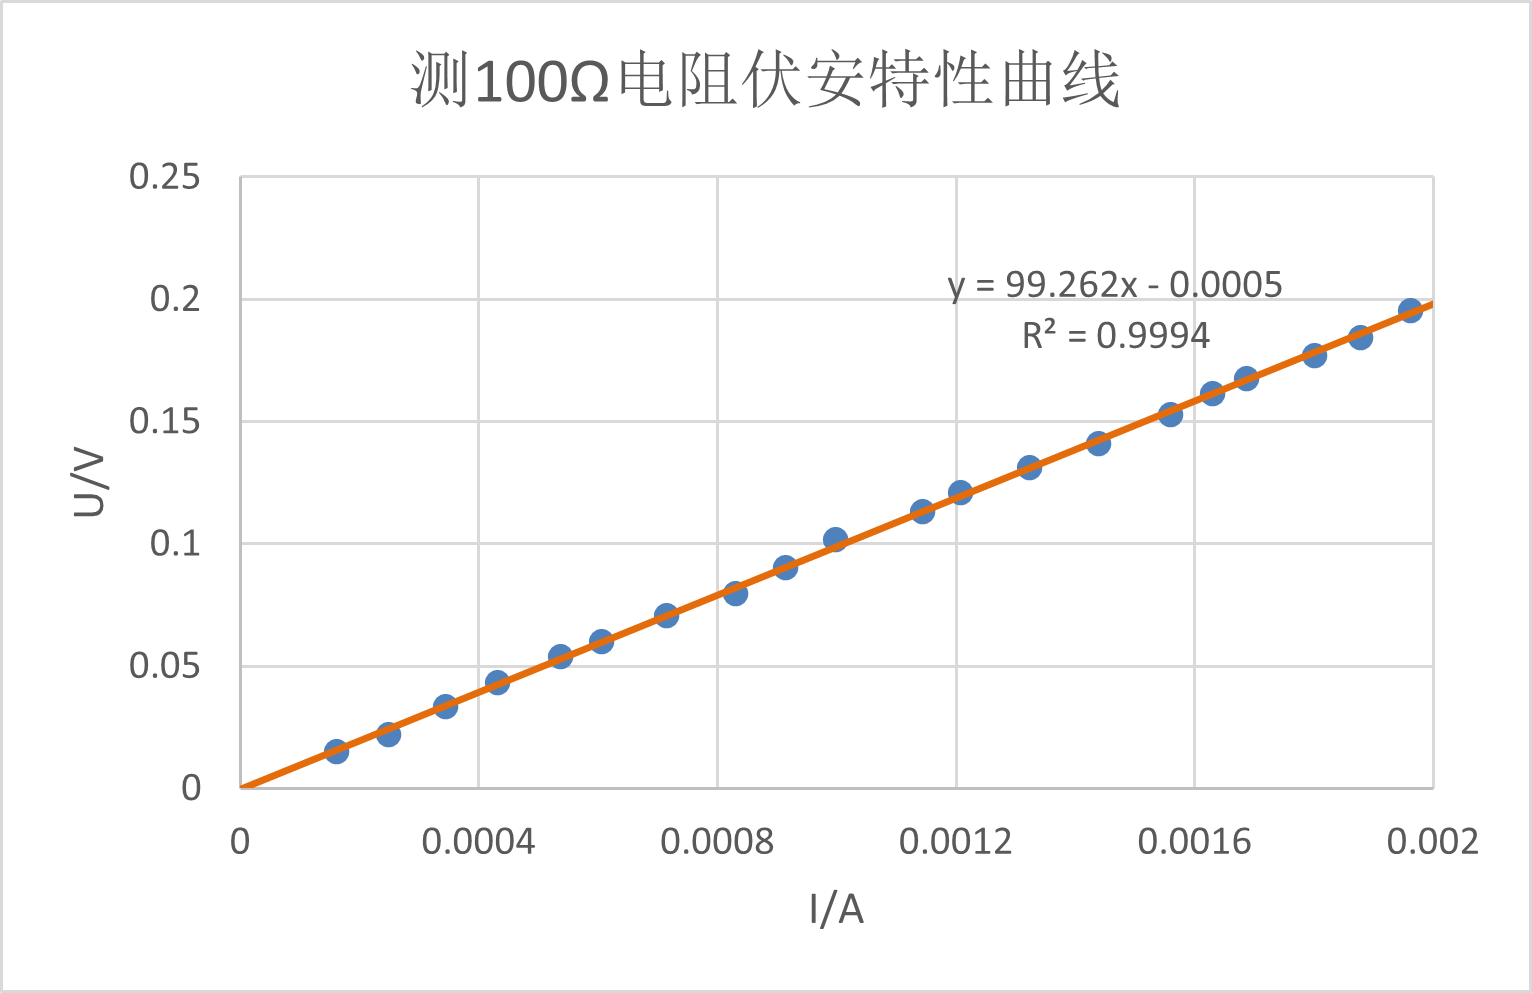
\includegraphics[width=8cm]{Fig/8.png} 
        }
        \subfigure[$10k\Omega$电阻伏安特性曲线]
        {   
            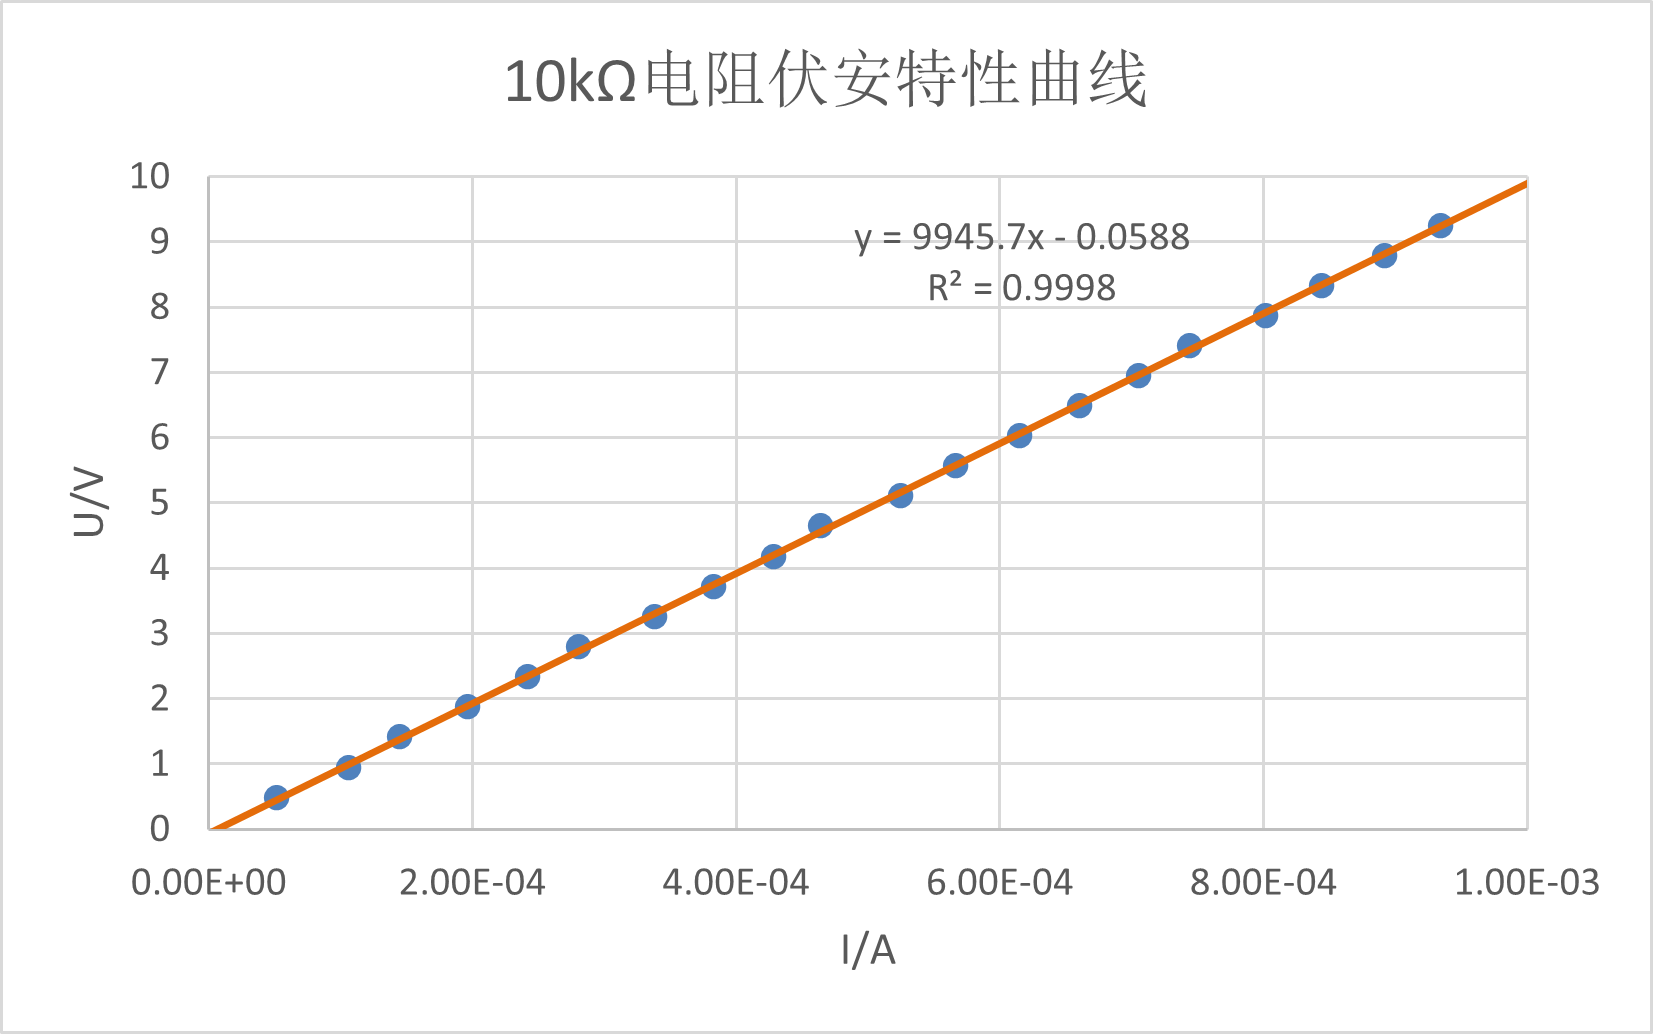
\includegraphics[width=8cm]{Fig/9.png}  
        }
        \subfigure[发光二极管伏安特性曲线]
        {
            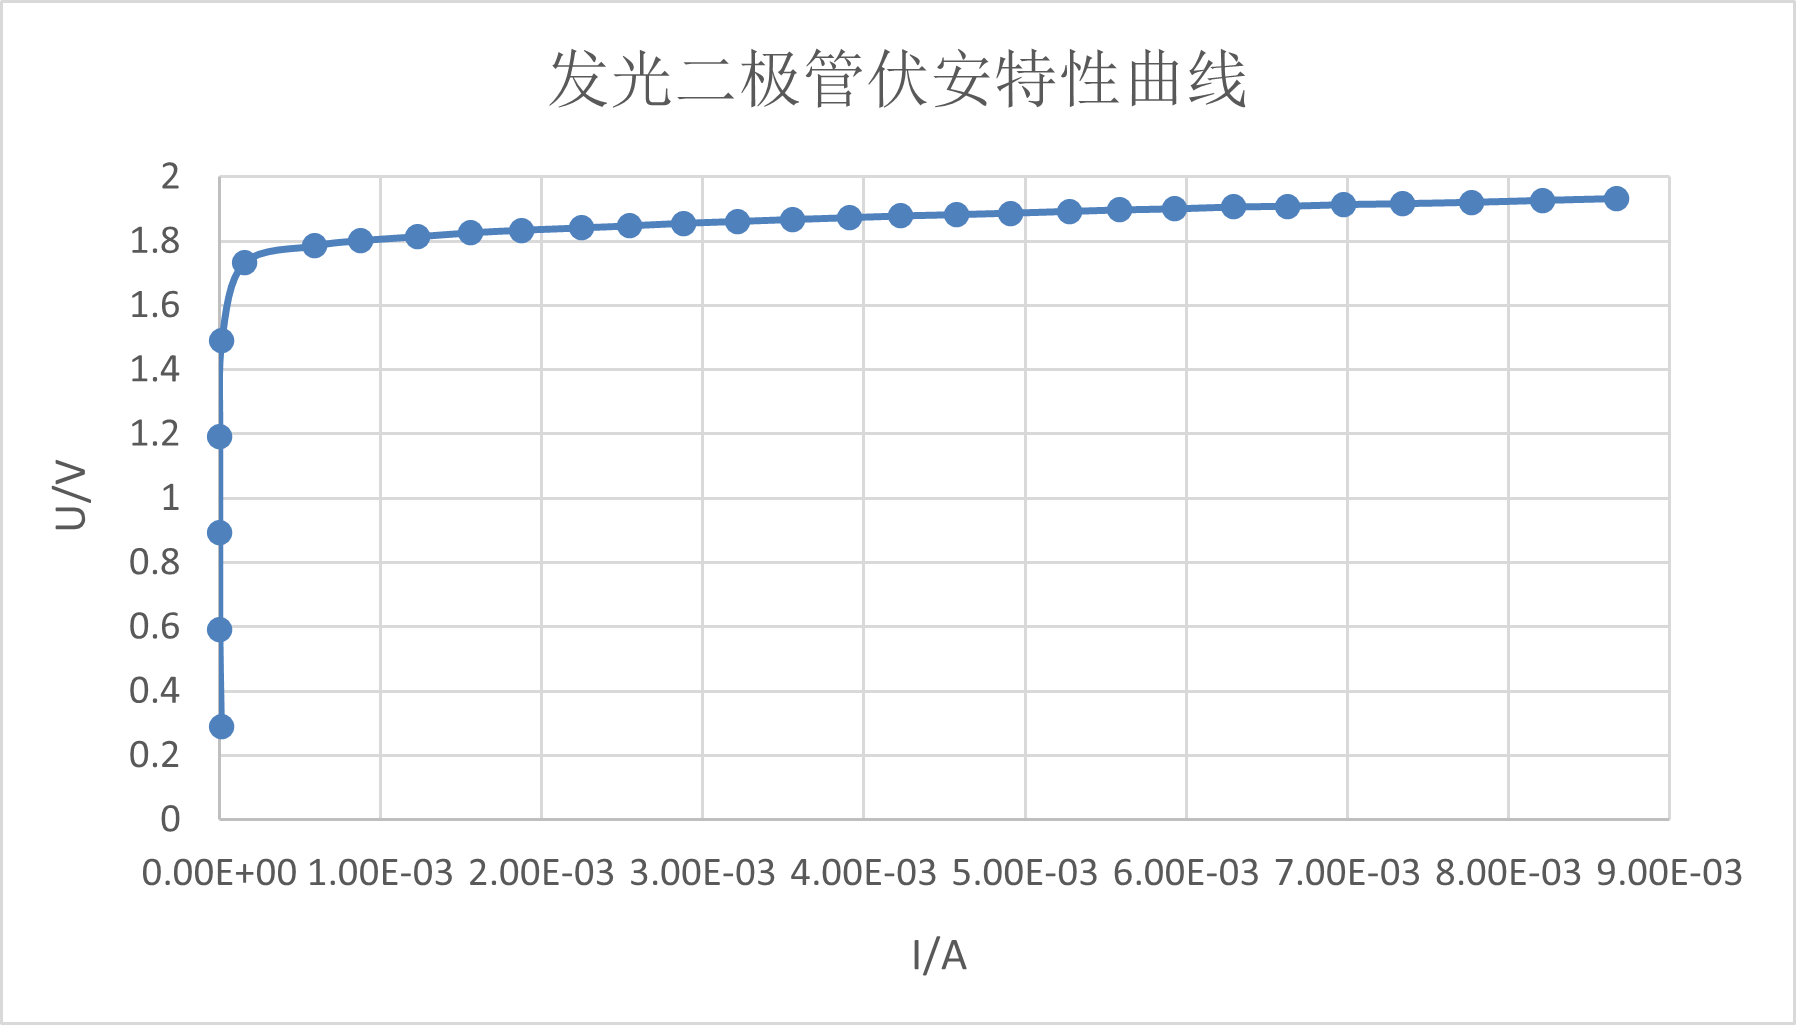
\includegraphics[width=8cm]{Fig/10.png} 
        }
        \caption{伏安特性曲线图}
       
    \end{figure}
\end{enumerate}

\subsection{实验反思,收获与总结}
\begin{enumerate}
    \item 思考题
    \begin{enumerate}
        \item 虚拟仪器系统与传统仪器有什么区别?请简要说明。
        \newline \hspace*{2em}虚拟仪器集成多种输入与输出,配合相应程序后能够有极多测量方案,泛用性强。虚拟仪器输出精度和测量电压精度较高,测量数据过小时自动转化为科学计数法,不像传统仪器需要考虑测量的量程。虚拟仪器内部集成示波器与信号发生器,在一定精度要求下能够做关于电波的实验,但高精度要求下传统设备处理输入波的能力更强。虚拟仪器程序中自带数据处理的控件,功能更强大。虚拟仪器将“仪器”装入“计算机”中,体现“软件指导硬件”的新概念。
        虚拟仪器的线路集成在仪器内部,难老化。
        \newline \hspace*{2em}在各种极端条件下,虚拟仪器测量效果差。虚拟仪器相对于传统仪器,泛用性强,但是在专门某方面的测量效果远远不如传统仪器。在做一些环境条件较温和的电学实验下,虚拟仪器较为好用。
        \item 本实验内容 3 中的电压输出和采集哪个先执行?
        \newline \hspace*{2em}类比传统仪器,应先电压输出,后采集。实际上在程序中两操作几乎同时开始,没有先后顺序区别。
    \end{enumerate}
    \item 误差分析
    \begin{enumerate}
        \item 本实验的测量精度相当高,可基本忽略测量误差。在实验4电压步进时,可以看到电压未准确地按照设置步长前进,但是测量点的数据仍旧准确,不影响测量。
        \item 过程中线阻可忽略。
        \item 由于仪器最大电流控制在$10mA$,量程较短,但在加入标准电阻进行分压后量程正常。
    \end{enumerate}
    \item 反思与收获
    \begin{enumerate}
        \item 虚拟仪器示波器相对于传统仪器示波器,调整空间小,仅作为示意图。传统示波器功能更全面更强大,对输入波的抗干扰性更强。
        \item 编程时注意细节与逻辑,某种程度上图形化编程仅仅减小上手成本,长期使用下并不好用。如果结合图形化编程与代码编程一体化,两者可以相互转化的情况下,会更利于工程测量。
        \item 测量伏安特性曲线时,要预估待测体电阻范围,设置合适的输出电压步长。实际操作中,当输出电压步长过大时,将限流,测量点将集中在尾部,为无效测量。程序中的示波器能够明显展示出此现象。
        \item 事实上,本人相当不信任虚拟仪器,如果输入和输出都是虚拟的,如实验2,在我无法拆解仪器确定内部线路连接的情况下,如何确定我所得的数据不是计算机杜撰的而是真实测量的?若程序出现难以察觉的错误导致严重误差,真的能说明实验结果吗?在一些实验中,异常数据反而能够推导出新的结论,但在模拟输出下,我们还能找到传统仪器下的异常数据吗?我还是更信任各类传统仪器,尽管有一些的误差是相当大的,如万用表。
    \end{enumerate}
\end{enumerate}




\end{document}